\documentclass[../Assignment-3-LPSMT.tex]{subfiles}
\graphicspath{{\subfix{../img/}}}

\begin{document}

\chapter{Implementazione}

Manga-check è stata sviluppata seguendo un modello a singola Activity con un
\href{https://developer.android.com/guide/navigation}{controller di navigazione}
che funge da istanziatore e sistema di passaggio di parametri da un fragment ad un altro.\\

\section{Divisione in moduli}

\section{Struttura del DB}

\lstinputlisting[language=Kotlin, caption={Parte di Series.kt}]{snippet-codice/Series.kt}

\lstinputlisting[language=Kotlin, caption={Parte di Chapter.kt}]{snippet-codice/Chapter.kt}

Nella definizione di Chapter abbiamo usato l'attributo \texttt{unique} per poter poi verificare la presenza di numeri duplicati e quindi fermare l'utente dall'inserimento.

\section{Richieste API}

Le richieste API sono state gestite con il sopracitato package \emph{ktor}, una parte della formattazione delle rispose alle API è stata gestita lato server per ridurre il codice da scrivere nell'applicazione e non sprecare rallentare troppo l'app.\\
Per gestire le risposte al meglio abbiamo di deciso di gestire lato client come delle matrici di stringhe.\\
Nel caso sottostante riceviamo i dati come una stringa che poi viene separata grazie ad una regex ed in seguito inserita in una matrice $[n][2]$ in cui $[n][0]$ contiene l'id del manga richiesto mentre $[n][1]$ il nome.

\begin{center}
  \includegraphics[scale=0.5]{queryNames.png}
  \captionof{figure}{Query dei vari nomi possibili per il manga}
\end{center}

\section{Uso di Safe Args}

Nel progetto abbiamo dovuto trasferire alcuni dati tra due fragment, come indicato nella documentazione Android abbiamo deciso di usare il \emph{navigation graph}, quindi vincolando i dati ad avere un determinato tipo.\\
Questo vincolo è stato possibile grazie all'utilizzo del plug in \href{https://developer.android.com/guide/navigation/use-graph/pass-data#Safe-args}{Safe Args} che ci ha permesso di specificare delle \emph{action} con un paylod di dati tipizzati.\\

\begin{center}
  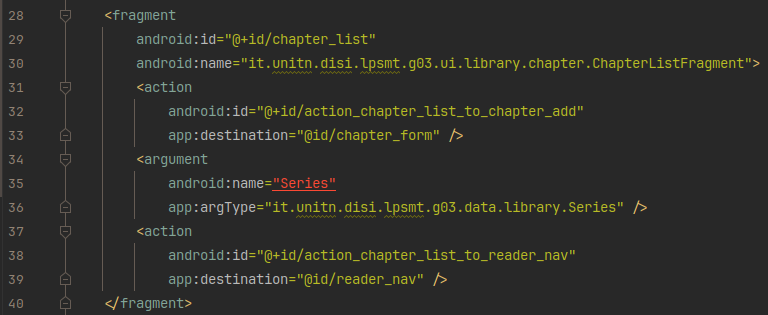
\includegraphics[scale=0.5]{action_navgraph.png}
  \captionof{figure}{Esempio di action con Safe Args}
\end{center}

\section{Backup Del DB}

Utilizzando le \href{https://developer.android.com/guide/topics/data/autobackup}{funzionalità native} di Android abbiamo implementato un sistema di Backup che permette all'utente di spostare la reading list senza bisogno di esportare alcun file.\\
%Sfruttato la funzionalità di cache abbiamo salvato le immagini di copertina dei comic in library e reding list, ed anche una versione decompressa del file \emph{cbz} da leggere.

\section{Reader}

I \emph{cbz} vengono prima decompressi in cache, cosi da non occupare troppa RAM, una volta fatto ciò, i file vengono converti durante l'esecuzione in Bitmap ridimensionate per coprire più superficie possibile.\\
Successivamente le Bitmap vengono associate ad una ImageView che si occupa di mostrarle all'utente.\\
Nel fragment del reader abbiamo implementato anche un bottone di ricerca per navigare più agevolmente all'interno del comic e due bottoni per muoversi tra le tavole.

\end{document}
